% Front and back cover pages for the white-paper book (kultem colours).
% Front image: 3.5ST_in_space.png   Back image: 3.5ST_in_KASI.png

\newcommand{\MakeFrontCover}{%
  \begin{titlepage}
  \thispagestyle{empty}\sffamily\centering
  % --- title banner ---
  \noindent\colorbox{Blue3}{\parbox[t]{\dimexpr\textwidth-2\fboxsep\relax}{%
    \vspace{4mm}\centering
    {\color{white}\bfseries\fontsize{24}{29}\selectfont 3.5-meter Segmented-Mirror\\[1.5mm]
      Robotic Space Telescope}\\[3.5mm]
    {\color{white}\Large Mission White Paper}\\[1.5mm]
    {\color{white!88}\large I. Overall Architecture and Scientific Mission}%
    \vspace{4mm}}}
  \vfill
  % --- cover image ---
% 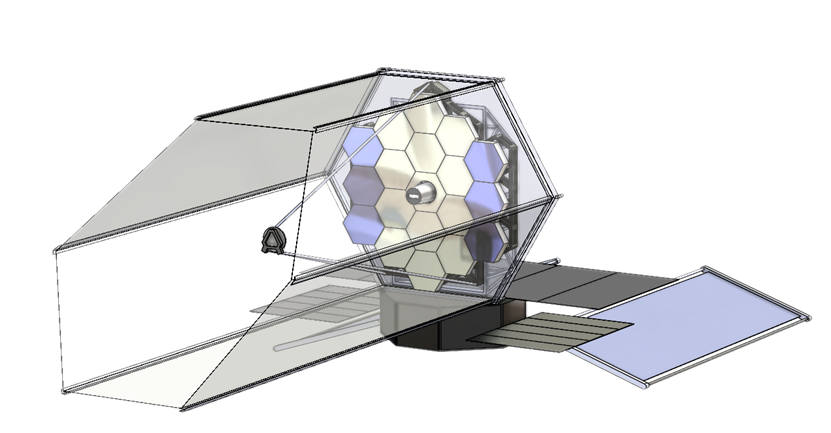
\includegraphics[width=\textwidth]{3.5ST_in_space.png}
  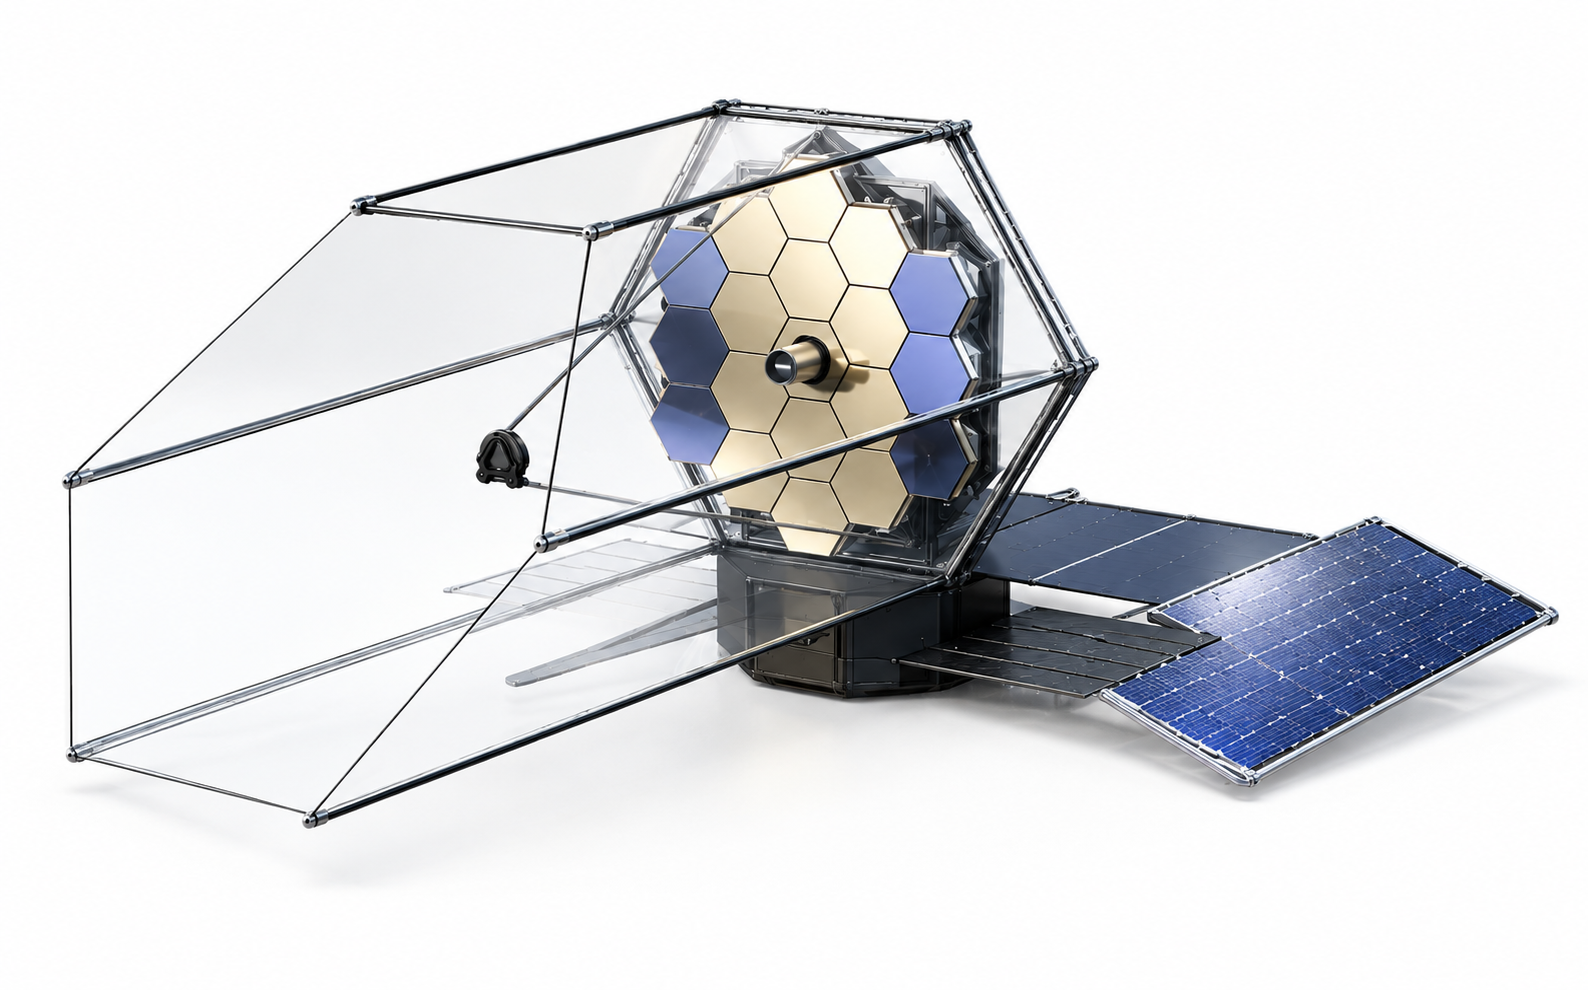
\includegraphics[width=\textwidth]{vol1_3.5ST_GPT.png}
  \vfill
  % --- authors and affiliations ---
  {\color{ink}\bfseries\normalsize \wpauthors\par}
  \vspace{3mm}
  {\color{muted}\small 
    Korea Astronomy and Space Science Institute \textperiodcentered\   
    University of Ulsan \\ 
    University of Science and Technology \textperiodcentered\
    Kyungpook National University\\
    Space Telescope Science Institute \textperiodcentered\ 
    Korea Institute for Advanced Study \\ 
    Pusan National University \textperiodcentered\ 
    Korea National University of Education\\
    Seoul National University \textperiodcentered\
    Yonsei University
    \par}
    
  \vspace{5mm}
  {\color{Blue3}\bfseries\Large 2026}
  \vspace{4mm}
  \end{titlepage}}

% Inside front cover: copyright / distribution notice / citation (colophon).
\newcommand{\MakeColophon}{%
  \clearpage
  \thispagestyle{empty}\sffamily
  \null\vfill
  \noindent{\color{muted}\footnotesize  
    {\color{ink}\bfseries 3.5-meter Segmented-Mirror Robotic Space Telescope}\\
    Mission White Paper: I. Overall Architecture and Scientific Mission\\[5mm]
%
    {\color{rose}\bfseries Release date September 2, 2026 \\ \\}
%    {\color{rose}\bfseries Draft for internal review --- not for public
%      distribution. \\ \\
%      June 20, 2026  First English draft \\
%      July 12, 2026  First LaTeX version \\
%      July 26, 2026  Revised version \\
%      August 5, 2026  Revised version \\
%     }\\[5mm]
%
    \textcopyright\ 2026 The 3.5mST Mission Study Team and the authors. All rights reserved.
    \\[2mm]
    Prepared by a community-based mission study team consisting of astronomers and researchers from multiple institutions in Korea and abroad.
    \\[5mm]
    {\color{ink}\bfseries Suggested citation:}\ Kang, Y.-W., Lee, S.-H., et
    al.\ (2026), \textit{3.5-meter Segmented-Mirror Robotic Space Telescope:
    Mission White Paper}.\\[2mm]
    {\color{ink}\bfseries Corresponding author:}\ Sang Hyun Lee
    \textperiodcentered\ \texttt{shlee@kasi.re.kr}.\\[5mm]
    {\color{ink}\bfseries AI-Assisted Illustrations:}\ Generative-AI tools were used solely for illustrative purposes in selected images in this white paper. AI-generated illustrations include the small illustrative images on pp. ii--iv and Figures 4.1, 4.3 (right panel), 4.4, and 4.5. The cover illustration was originally created by a human designer and subsequently retouched using AI-assisted image tools. Generative AI was not used to produce scientific data, observational results, quantitative simulations, or scientific measurements presented in this white paper. All externally sourced scientific images and data are credited to their original sources where applicable.
    \\[5mm]
    
%    Typeset in \LaTeX\ with the \textsf{kultem} style. Version: draft, 2026.
    \par}
  \vspace{8mm}
  \clearpage}

\newcommand{\MakeBackCover}{%
  % the inside back cover (blank verso before the cover) must fall on an
  % odd (recto) page for correct two-sided binding; add a filler if needed
%  \clearpage
%  \ifodd\value{page} \hbox{}\thispagestyle{empty}\newpage \fi
%  \thispagestyle{empty}\null      % inside back cover (blank), on an odd page
%  \clearpage
  \thispagestyle{empty}\sffamily\centering
  
  \null\vspace*{\stretch{1}}
%  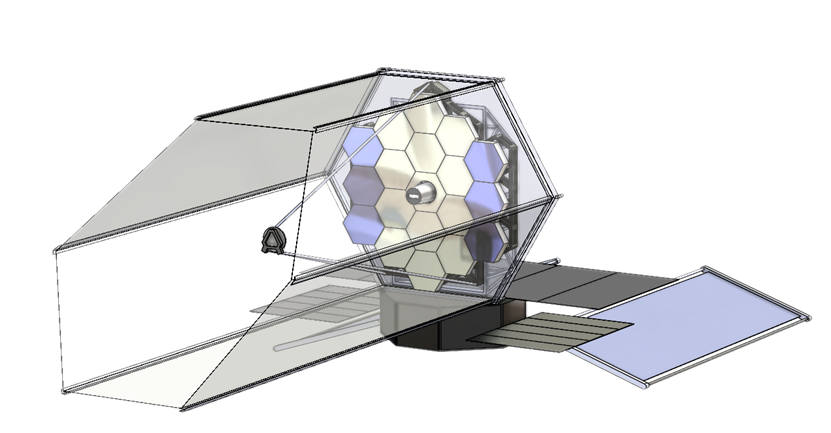
\includegraphics[width=\textwidth]{3.5ST_in_KASI.png}
  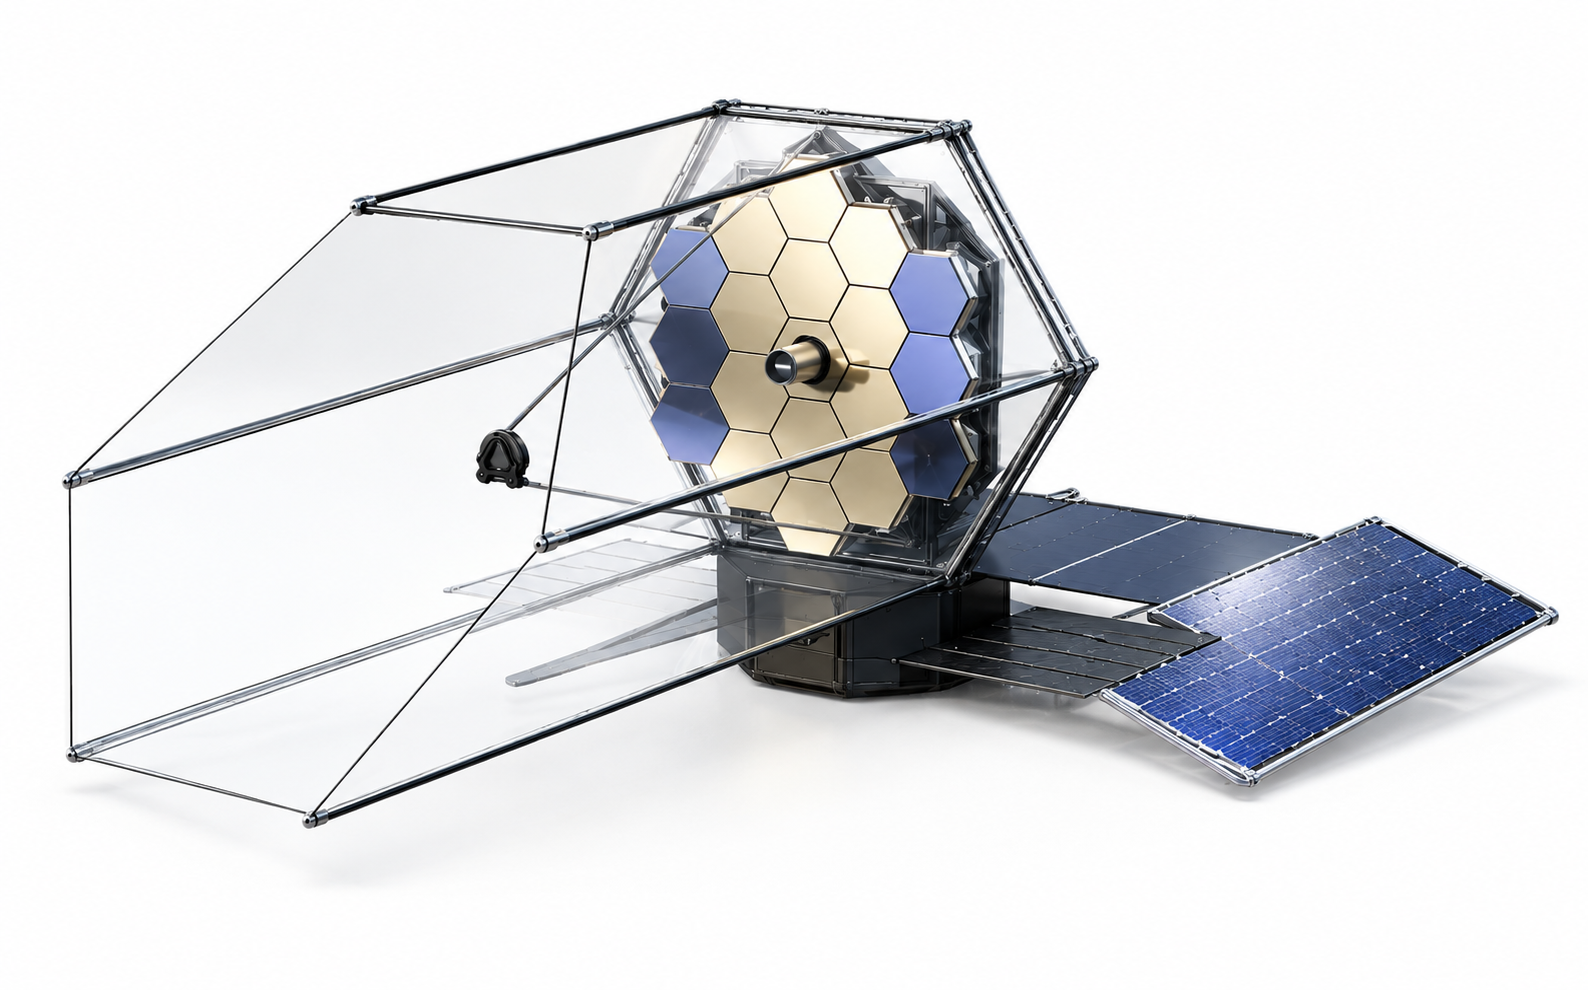
\includegraphics[width=\textwidth]{vol1_3.5ST_GPT.png}
  \vspace*{\stretch{2.2}}
  \noindent\colorbox{Blue3}{\parbox[t]{\dimexpr\textwidth-2\fboxsep\relax}{%
    \vspace{3mm}\centering
    {\color{white}\bfseries\Large 3.5-meter Segmented-Mirror Robotic Space Telescope}\\[1.5mm]
    {\color{white!88}\normalsize Mission White Paper: I. Overall Architecture and Scientific Mission}%
    \vspace{3mm}}}
  \vspace{3mm}
  \clearpage}
